\section{Initial set of rectangles}

We present a set of rectangles
whose projections cover the segment from the Freiman's constant to $\sqrt{21}$.
All of them are good.
Further sections will present the algorithm of splitting these rectangles into subrectangles correctly.

\begin{figure}[H]
	\centering
	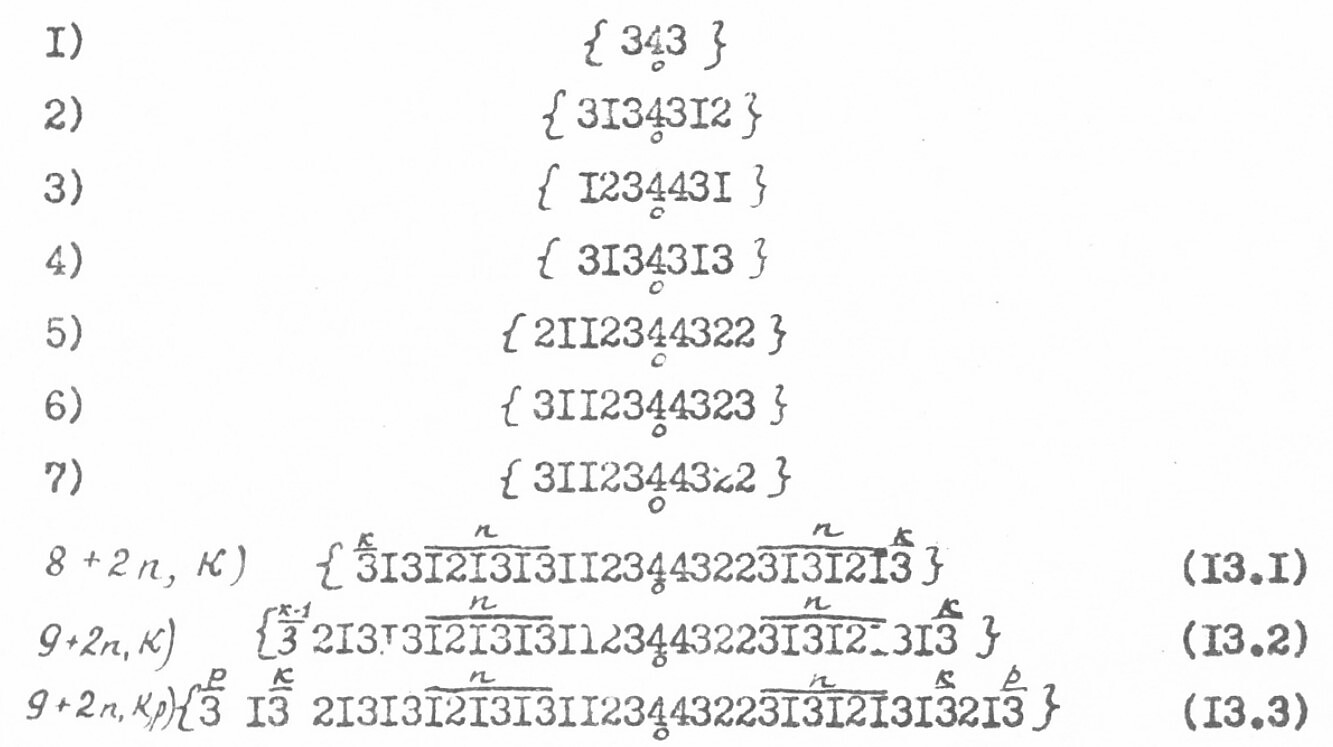
\includegraphics[width=0.8\textwidth]{initial-set}
	\caption{Initial set of rectangles.}
	\label{initial-set}
\end{figure}

The segments covered by these rectangles are presented in the table below:

\begin{figure}[H]
	\centering
	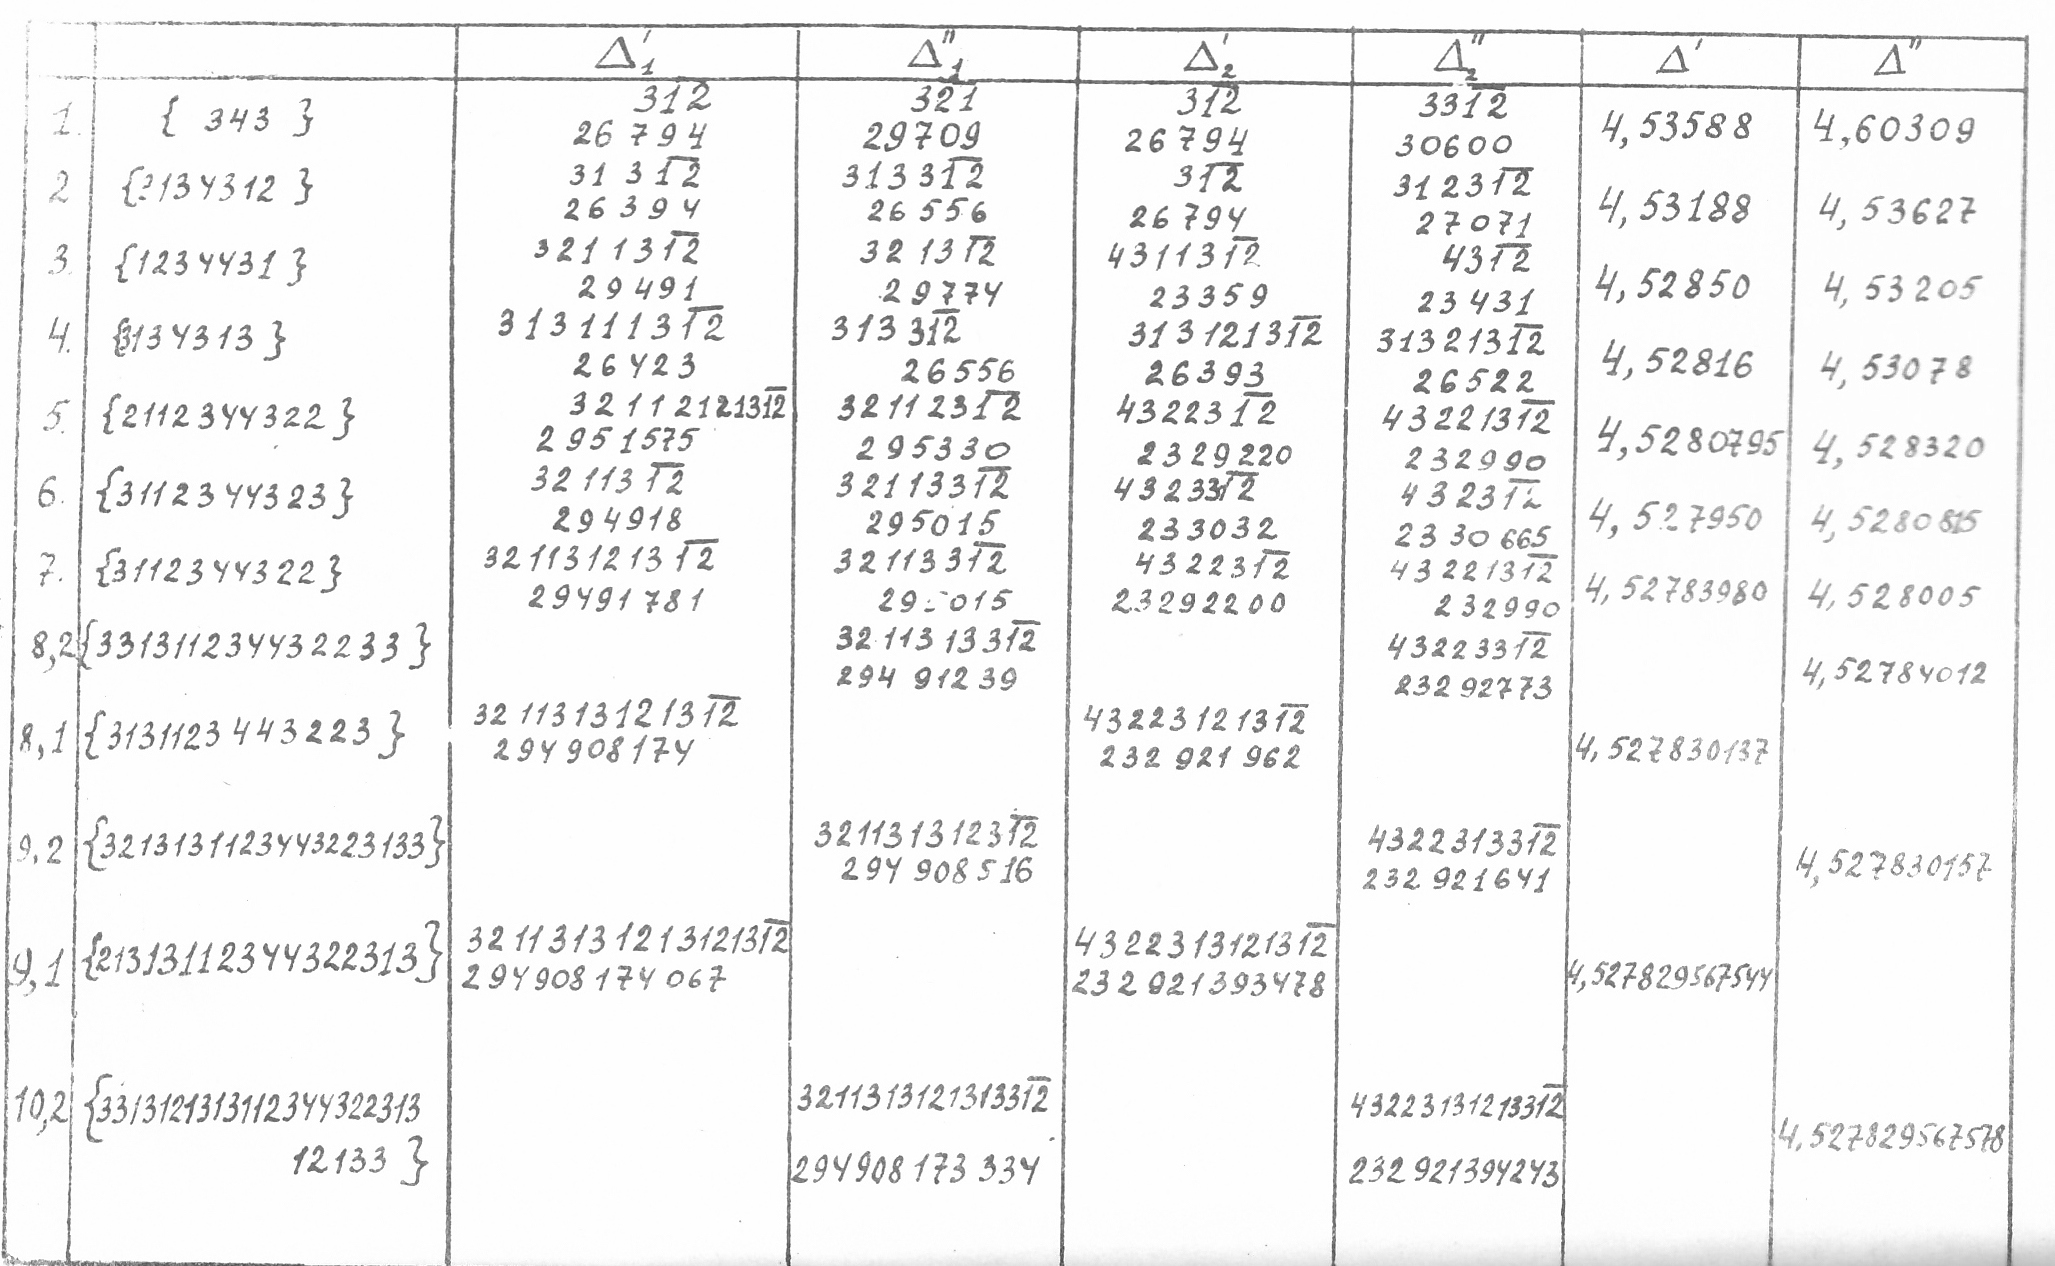
\includegraphics[width=\textwidth]{initial-set-boundaries}
	\caption{Segments covered by rectangles.}
	\label{initial-set-table}
\end{figure}